% Source for the figure of offlineConnectivity (sec. 11.5): the segment
% tree over q = 4 questions, and the nodes that hold an edge alive from the
% question 1 to the end, i.e., on the times [1, 4): the leaf [1, 2) and
% the node [2, 4). Build: make figures (in ../build).
\documentclass[border=4pt]{standalone}
\usepackage[T1]{fontenc}
\usepackage{lmodern}
\usepackage{amsmath,amssymb}
\usepackage{tikz}
\usepackage{lamalunga}
% tikz-ads.tex: the TikZ styles shared by the figures of the memory of the
% manual, \input by each standalone figure: a cell of a vector (cell), the
% cell that an operation touches (touched), a free cell (free), a node of a
% linked structure (node), the labels of indices (index) and of variables
% (var), a pointer (ptr), and \cells and \indices to draw a row of cells.
\usetikzlibrary{arrows.meta,positioning,calc,fit,shapes.multipart}
\definecolor{adsTouched}{RGB}{214,196,236}
\definecolor{adsFree}{RGB}{236,236,236}
\tikzset{
  ads/.style={>={Stealth[length=2mm]},font=\small,
              every node/.append style={inner sep=0pt}},
  cell/.style={draw,minimum width=7mm,minimum height=7mm,
               font=\small\ttfamily,outer sep=0pt},
  touched/.style={cell,fill=adsTouched},
  free/.style={cell,fill=adsFree,text=black!45},
  node/.style={draw,rounded corners=1pt,minimum width=8mm,
               minimum height=6mm,font=\small\ttfamily},
  index/.style={font=\scriptsize\ttfamily,text=black!60},
  var/.style={font=\small\itshape},
  ptr/.style={->,thick}
}
% \cells{name}{x,y}{list}: a row of cells, the first at (x,y), named
% name-0, name-1, ...; each item is text/style, the style one of cell,
% touched and free (e.g., {a/cell,e/touched,/free})
\newcommand{\cells}[3]{%
  \foreach \v/\s [count=\i from 0] in {#3}
    \node[\s] (#1-\i) at ($(#2)+(\i*7mm,0)$) {\v};}
% \indices{name}{n}: the indices 0 .. n-1 under the cells of name
\newcommand{\indices}[2]{%
  \foreach \i in {0,...,\numexpr#2-1\relax}
    \node[index,below=1.2mm of #1-\i] {\i};}

\tikzset{s/.style={draw,rounded corners=1pt,minimum width=14mm,
  minimum height=6mm,font=\small}}
\begin{document}
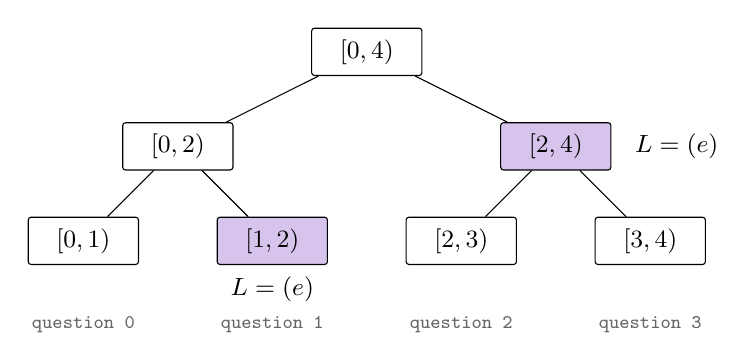
\begin{tikzpicture}[ads]
  \node[s] (r) at (0,0) {$[ 0 , 4 )$};
  \node[s] (l) at (-24mm,-12mm) {$[ 0 , 2 )$};
  \node[s,fill=adsTouched] (h) at (24mm,-12mm) {$[ 2 , 4 )$};
  \node[s] (l0) at (-36mm,-24mm) {$[ 0 , 1 )$};
  \node[s,fill=adsTouched] (l1) at (-12mm,-24mm) {$[ 1 , 2 )$};
  \node[s] (h0) at (12mm,-24mm) {$[ 2 , 3 )$};
  \node[s] (h1) at (36mm,-24mm) {$[ 3 , 4 )$};
  \draw (r) -- (l); \draw (r) -- (h);
  \draw (l) -- (l0); \draw (l) -- (l1); \draw (h) -- (h0); \draw (h) -- (h1);
  \node[var,anchor=west] at (34mm,-12mm) {$L = ( e )$};
  \node[var,anchor=north] at (-12mm,-28.5mm) {$L = ( e )$};
  \foreach \n/\i in {l0/0,l1/1,h0/2,h1/3}
    \node[index,anchor=north] at ($(\n.south)+(0,-6.5mm)$) {question \i};
\end{tikzpicture}
\end{document}
